% -*- coding: utf-8 -*-
% Синтаксически рекурсивный факториал
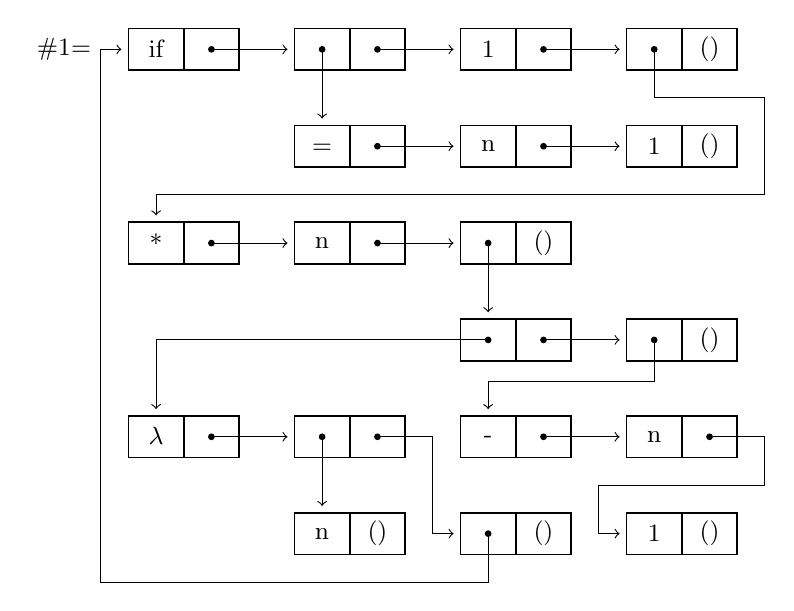
\begin{tikzpicture}
  \tikzstyle{every node}=[font=\small]

% (if ... 1 ...)
  \draw (-1.0em, -0.75em) node[left] {\ic{\#1=}};

  \draw [semithick] ( 0.0em,  0.0em) rectangle  ( 4.0em, -1.5em);
  \draw [semithick] ( 2.0em,  0.0em) -- ( 2.0em, -1.5em);

  \draw [semithick] ( 6.0em,  0.0em) rectangle  (10.0em, -1.5em);
  \draw [semithick] ( 8.0em,  0.0em) -- ( 8.0em, -1.5em);

  \draw [semithick] (12.0em,  0.0em) rectangle  (16.0em, -1.5em);
  \draw [semithick] (14.0em,  0.0em) -- (14.0em, -1.5em);

  \draw [semithick] (18.0em,  0.0em) rectangle  (22.0em, -1.5em);
  \draw [semithick] (20.0em,  0.0em) -- (20.0em, -1.5em);

  \filldraw  ( 3.0em, -0.75em) circle(1.0pt);
  \draw [->] ( 3.0em, -0.75em) -- ( 5.75em, -0.75em);

  \filldraw  ( 9.0em, -0.75em) circle(1.0pt);
  \draw [->] ( 9.0em, -0.75em) -- (11.75em, -0.75em);

  \filldraw  (15.0em, -0.75em) circle(1.0pt);
  \draw [->] (15.0em, -0.75em) -- (17.75em, -0.75em);

  \filldraw  ( 7.0em, -0.75em) circle(1.0pt);
  \draw [->] ( 7.0em, -0.75em) -- ( 7.00em, -3.25em);

  \filldraw  (19.0em, -0.75em) circle(1.0pt);
  \draw [->] (19.0em, -0.75em) -- (19.00em, -2.50em) --
             (23.0em, -2.50em) -- (23.00em, -6.00em) --
             ( 1.0em, -6.00em) -- ( 1.00em, -6.75em);

  \draw ( 1.0em, -0.75em) node {\ic{if}};
  \draw (13.0em, -0.75em) node {\ic{1}};
  \draw (21.0em, -0.75em) node {\ic{()}};

% (= n 1)
  \draw [semithick] ( 6.0em, -3.5em) rectangle  (10.0em, -5.0em);
  \draw [semithick] ( 8.0em, -3.5em) -- ( 8.0em, -5.0em);

  \draw [semithick] (12.0em, -3.5em) rectangle  (16.0em, -5.0em);
  \draw [semithick] (14.0em, -3.5em) -- (14.0em, -5.0em);

  \draw [semithick] (18.0em, -3.5em) rectangle  (22.0em, -5.0em);
  \draw [semithick] (20.0em, -3.5em) -- (20.0em, -5.0em);

  \filldraw  ( 9.0em, -4.25em) circle(1.0pt);
  \draw [->] ( 9.0em, -4.25em) -- (11.75em, -4.25em);

  \filldraw  (15.0em, -4.25em) circle(1.0pt);
  \draw [->] (15.0em, -4.25em) -- (17.75em, -4.25em);

  \draw ( 7.0em, -4.35em) node {\ic{=}};
  \draw (13.0em, -4.25em) node {\ic{n}};
  \draw (19.0em, -4.25em) node {\ic{1}};
  \draw (21.0em, -4.25em) node {\ic{()}};

% (* n ...)
  \draw [semithick] ( 0.0em, -7.0em) rectangle  ( 4.0em, -8.5em);
  \draw [semithick] ( 2.0em, -7.0em) -- ( 2.0em, -8.5em);

  \draw [semithick] ( 6.0em, -7.0em) rectangle  (10.0em, -8.5em);
  \draw [semithick] ( 8.0em, -7.0em) -- ( 8.0em, -8.5em);

  \draw [semithick] (12.0em, -7.0em) rectangle  (16.0em, -8.5em);
  \draw [semithick] (14.0em, -7.0em) -- (14.0em, -8.5em);

  \filldraw  ( 3.0em, -7.75em) circle(1.0pt);
  \draw [->] ( 3.0em, -7.75em) -- ( 5.75em, -7.75em);

  \filldraw  ( 9.0em, -7.75em) circle(1.0pt);
  \draw [->] ( 9.0em, -7.75em) -- (11.75em, -7.75em);

  \filldraw  (13.0em, -7.75em) circle(1.0pt);
  \draw [->] (13.0em, -7.75em) -- (13.00em,-10.25em);

  \draw ( 1.0em, -7.75em) node {\ic{*}};
  \draw ( 7.0em, -7.75em) node {\ic{n}};
  \draw (15.0em, -7.75em) node {\ic{()}};

% (... ...)
  \draw [semithick] (12.0em,-10.5em) rectangle  (16.0em,-12.0em);
  \draw [semithick] (14.0em,-10.5em) -- (14.0em,-12.0em);

  \draw [semithick] (18.0em,-10.5em) rectangle  (22.0em,-12.0em);
  \draw [semithick] (20.0em,-10.5em) -- (20.0em,-12.0em);

  \filldraw  (15.0em, -11.25em) circle(1.0pt);
  \draw [->] (15.0em, -11.25em) -- (17.75em, -11.25em);

  \filldraw  (19.0em, -11.25em) circle(1.0pt);
  \draw [->] (19.0em, -11.25em) -- (19.00em, -12.75em) --
             (13.0em, -12.75em) -- (13.00em, -13.75em);

  \filldraw  (13.0em, -11.25em) circle(1.0pt);
  \draw [->] (13.0em, -11.25em) -- ( 1.00em, -11.25em) -- (1.00em, -13.75em);

  \draw (21.0em, -11.25em) node {\ic{()}};

% (lambda ... #1)   (- n ...)
  \draw [semithick] ( 0.0em,-14.0em) rectangle  ( 4.0em,-15.5em);
  \draw [semithick] ( 2.0em,-14.0em) -- ( 2.0em,-15.5em);

  \draw [semithick] ( 6.0em,-14.0em) rectangle  (10.0em,-15.5em);
  \draw [semithick] ( 8.0em,-14.0em) -- ( 8.0em,-15.5em);

  \draw [semithick] (12.0em,-14.0em) rectangle  (16.0em,-15.5em);
  \draw [semithick] (14.0em,-14.0em) -- (14.0em,-15.5em);

  \draw [semithick] (18.0em,-14.0em) rectangle  (22.0em,-15.5em);
  \draw [semithick] (20.0em,-14.0em) -- (20.0em,-15.5em);

  \filldraw  ( 3.0em, -14.75em) circle(1.0pt);
  \draw [->] ( 3.0em, -14.75em) -- ( 5.75em, -14.75em);

  \filldraw  (15.0em, -14.75em) circle(1.0pt);
  \draw [->] (15.0em, -14.75em) -- (17.75em, -14.75em);

  \filldraw  ( 7.0em, -14.75em) circle(1.0pt);
  \draw [->] ( 7.0em, -14.75em) -- ( 7.00em, -17.25em);

  \filldraw  (21.0em, -14.75em) circle(1.0pt);
  \draw [->] (21.0em, -14.75em) -- (23.00em, -14.75em) --
             (23.0em, -16.50em) -- (17.00em, -16.50em) --
             (17.0em, -18.25em) -- (17.75em, -18.25em);

  \filldraw  ( 9.0em, -14.75em) circle(1.0pt);
  \draw [->] ( 9.0em, -14.75em) -- (11.00em, -14.75em) --
             (11.0em, -18.25em) -- (11.75em, -18.25em);

  \draw ( 1.0em, -14.70em) node {$\lambda$};
  \draw (13.0em, -14.75em) node {\ic{-}};
  \draw (19.0em, -14.75em) node {\ic{n}};

% (n)   (#1#)   (... 1)
  \draw [semithick] ( 6.0em,-17.5em) rectangle  (10.0em,-19.0em);
  \draw [semithick] ( 8.0em,-17.5em) -- ( 8.0em,-19.0em);

  \draw [semithick] (12.0em,-17.5em) rectangle  (16.0em,-19.0em);
  \draw [semithick] (14.0em,-17.5em) -- (14.0em,-19.0em);

  \draw [semithick] (18.0em,-17.5em) rectangle  (22.0em,-19.0em);
  \draw [semithick] (20.0em,-17.5em) -- (20.0em,-19.0em);

  \filldraw  (13.00em, -18.25em) circle(1.0pt);
  \draw [->] (13.00em, -18.25em) -- (13.00em, -20.00em) --
             (-1.00em, -20.00em) -- (-1.00em,  -0.75em) -- (-0.25em, -0.75em);

  \draw ( 7.0em, -18.25em) node {\ic{n}};
  \draw ( 9.0em, -18.25em) node {\ic{()}};
  \draw (15.0em, -18.25em) node {\ic{()}};
  \draw (19.0em, -18.25em) node {\ic{1}};
  \draw (21.0em, -18.25em) node {\ic{()}};
\end{tikzpicture}
